\documentclass{article}
% \usepackage[landscape,a4paper, lmargin=10mm, rmargin=10mm, top=10mm, bottom=10mm]{geometry}
% \usepackage[portrait, a4paper, lmargin=10mm, rmargin=10mm, top=10mm, bottom=10mm]{geometry}
\usepackage[portrait, a4paper, margin=2mm]{geometry}
\usepackage{multicol}
\usepackage{lipsum} % zum Testen, kannst du später entfernen
\usepackage{titlesec}
\usepackage{enumitem}
\usepackage{xcolor}
\usepackage{setspace}
\pagestyle{empty}

% Layout-Anpassungen
\setstretch{0.9}
\setlength{\columnsep}{5mm}
\setlength{\columnseprule}{0.4pt}
\setlength{\parindent}{0pt}

% \newcommand{\var}{\textit{var}}
% \newcommand{\free}{\textit{free}}
\newcommand{\imp}[1]{{\color{red} #1}} % red text is important

\let\olditemize\itemize
\renewcommand{\itemize}{\olditemize[itemindent=1mm, topsep=0mm, leftmargin=2mm, labelsep=0.5mm, parsep=0mm, itemsep=0mm]}
\let\oldenumerate\enumerate
\renewcommand{\enumerate}{\oldenumerate[itemindent=1mm, topsep=0mm, leftmargin=2mm, labelsep=0.5mm, parsep=0mm, itemsep=0mm]}

\titleformat*\subsubsection{\scriptsize\bfseries}
\titlespacing*{\subsubsection}{0mm}{2mm}{1mm}


\begin{document}
% \small
% \footnotesize
\scriptsize
% \tiny

% -------- Seite 1: z.B. 5 Spalten --------
\begin{multicols}{4}
    % \subsubsection*{1a) Introduction}

% \textbf{What is an OS?} An intermediary between user and hardware. \textbf{Functions:} Resource allocator (resolves conflicts for fair and efficient resource use), control program (prevents errors, improper use). \textbf{Always running:} OS kernel. \textbf{Goals:} Program execution, user convenience, efficient hardware utilization. \textbf{Position:} Between hardware and user mode (kernel mode).

% \textbf{Components of a CS:}\\
% - \textbf{Hardware} provides basic computing resources (CPU, memory, I/O devices)\\
% - \textbf{OS} controls and coordinates use of hw among various apps and users\\
% - \textbf{App programs} define how system resources are used to solve user problems (web browsers, compilers, games)\\
% - \textbf{Users} (people, machines, other computers)\\

% \textbf{System organization:} Bus connects CPU, memory, and device controllers; concurrent execution leads to memory access competition. \textbf{I/O:} Local buffer in device controller, device driver (OS component), CPU moves data to/from main bus. Device signals completion via interrupt; ISR uses interrupt vector, returns control to CPU (resumes from saved instruction). OS is interrupt-driven.

% \textbf{Memory:} Main memory (volatile, programs/data); non-volatile storage (HDD: tracks/sectors, SSD). \textbf{Hierarchy:} Access time, capacity, cost, volatility. \textbf{Caching:} Stores data from slower memory into faster storage (size, policy, management important). \textbf{DMA:} Direct Memory Access—device buffer $\rightarrow$ memory without CPU.

% \textbf{Key terms:} CPU (executes instructions), Processor (chip with CPUs), Core (basic computation unit), Multicore (multiple cores per chip), Multiprocessor (multiple processors per system). \textbf{Types:} AMP (asymmetric—specialized CPUs), SMP (symmetric—CPUs share all tasks). \textbf{Memory:} Shared-memory systems; NUMA (non-uniform memory access); Clusters (multiple systems linked via LAN, AMP/SMP possible, HPC).

% \textbf{Boot process:} Bootstrap program (firmware in ROM/EPROM), initializes system, loads kernel. \textbf{Modes:} Batch (multiprogramming: job scheduling, no interactivity); Time-sharing (interactive, multiple jobs, CPU scheduling, swapping, virtual memory). Dual mode (user/kernel), privileged instructions only in kernel mode; syscalls switch to kernel, return sets user mode. Multi-mode via Virtual Machine Monitor (VMM). ARMv8: 7 modes. \textbf{Timer:} Interrupts to prevent user-mode lockups.

% \textbf{Resources:} Process (active unit, needs resources, cleaned up on termination); Program (passive entity). Multiplexing CPU across processes. OS handles process creation/termination, suspend/resume, sync, communication, deadlocks. \textbf{Memory management:} Manages what is in memory, allocates/deallocates space. \textbf{Storage:} OS abstracts storage (files, directories), controls access, manages file system, backups. \textbf{Virtualization:} Run OS within OS (VMM required). Emulation: for different CPU types; Virtualization: same CPU type.

% \textbf{Kernel data structures:} Lists (single/double/circular, $O(n)$); Stacks (LIFO, function calls); Queues (FIFO, task waiting); Trees (parent-child, binary, balanced $O(\log n)$); Hash tables ($O(1)$, with linked lists for collisions); Bitmaps (status of $n$ items, 1=unavailable).


% \subsubsection*{1b) History}

% \textbf{Gen 1 (1940-1955):} Vacuum tubes, no OS (user=operator), assembler, linker, inefficient (manual I/O, one job at a time).

% \textbf{Gen 2 (1955-1965):} Transistors, batch systems, control cards (job type, program info), first rudimentary OS (job sequencing). CPU idle during I/O. Spooling (offline I/O into tapes, overlapping I/O and computation).

% \textbf{Gen 3 (1965-1980):} Integrated circuits, multiprogramming, spooling to memory, memory partitioning, time-sharing (interactive users, CPU scheduling, swapping, memory management, synchronization, communication). \textbf{CTSS:} Time-sharing prototype (interactive users, multiple jobs). \textbf{MULTICS:} Predecessor to UNIX (hierarchical file system, protection rings). \textbf{UNIX:} Modular (everything is a file), multitasking, multiuser, in C, open source from 1994. \textbf{Parallel OS:} 1960s onward: shared-memory multiprocessors, asynchronous events, independent tasks.

% \textbf{Gen 4 (1980-present):} PCs, microkernels (e.g., MINIX3: fault tolerance, user-mode drivers), Windows (from DOS, GUI, client-server), macOS, Linux (free, UNIX-like, user-driven). \textbf{Linux versions:} 0.01 (no networking), 1.0 (TCP/IP, devices, filesystems), 1.2 (PC-only), 2.x (SMP, kernel threads, modules), 3.x (fair scheduler), 4.x (x86, I/O improvements), 5.x (scheduler cleanup), 6.x (performance improvements). \textbf{Networked OS:} Illusion of single system, own local OS, Network Interface Controller (NIC), remote access. \textbf{DOS (Distributed OS):} Multiple processors per application, user unaware of program location, complex scheduling, delays. \textbf{NOS (Network OS):} Client-server model; DOS: coordinator-worker model.

% \textbf{Gen 5 (1990-present):} Mobile computing: early heavy devices, 70s "the brick," 90s Nokia, 98 SymbianOS, 02 BlackBerry, 07 iOS, 08 Android, 11 Windows Phone.

% \textbf{Ontogeny Recapitulates Phylogeny:} OS design influenced by hardware capabilities. Obsolete concepts sometimes return (e.g., microkernels).

\subsubsection*{1a) Introduction}

\textbf{OS:} Intermediary between user and hardware. \textbf{Functions:} Resource allocator (fair use), control program (safe use), kernel always running. \textbf{Goals:} Execution, convenience, efficiency. \textbf{Position:} Between hardware and user mode (kernel mode).

\textbf{CS components:} \textbf{Hardware} (CPU, memory, I/O), \textbf{OS} (manage hw, apps, users), \textbf{Apps} (user solutions), \textbf{Users}.

\textbf{System:} Bus links CPU/memory/controllers; concurrent exec causes memory access conflicts. \textbf{I/O:} Device controller buffer, driver, interrupts (ISR, vector), OS is interrupt-driven. \textbf{Memory:} Main (volatile), storage (non-volatile); hierarchy: speed, size, cost. \textbf{Cache:} Faster store for slower memory. \textbf{DMA:} Device $\rightarrow$ memory (no CPU).

\textbf{Key terms:} CPU (executes), Processor (chip w/ CPUs), Core (unit), Multicore (cores/chip), Multiproc (CPUs/system). \textbf{Types:} AMP (specialized), SMP (equal tasks), NUMA (non-uniform memory), Clusters (LAN, AMP/SMP). 

\textbf{Boot:} Bootstrap (ROM/EPROM) loads kernel. \textbf{Modes:} Batch (jobs, no interactivity), Time-sharing (interactive, multiple jobs), Dual-mode (user/kernel, privileged instr), syscalls switch modes. Timer prevents lockups. VMM: multi-mode OS. ARMv8: 7 modes.

\textbf{Resources:} \textbf{Process} (active, needs resources), \textbf{Program} (passive). OS multiplexes CPU, manages process lifecycle, memory, files, devices. \textbf{Virtualization:} OS in OS (VMM), emulation for different CPUs.

\textbf{Kernel structures:} Lists ($O(n)$), Stacks (LIFO), Queues (FIFO), Trees ($O(\log n)$), Hash ($O(1)$), Bitmaps (status).

\subsubsection*{1b) History}

\textbf{Gen 1:} Vacuum tubes, no OS.\\
\textbf{Gen 2:} Batch systems, control cards, spooling (tape).\\
\textbf{Gen 3:} ICs, multiprogramming, spooling $\rightarrow$ memory, time-sharing (CTSS, MULTICS, UNIX: C, modular, open).\\
\textbf{Gen 4:} PCs, microkernels (MINIX), Windows, macOS, Linux (free, UNIX-like). Distributed systems: Network OS (NIC, client-server), Distributed OS (single system illusion).\\
\textbf{Gen 5:} Mobile: Nokia, Symbian, BB, iOS, Android.

\textbf{Ontogeny Recapitulates Phylogeny:} Hardware shapes OS; old concepts return (e.g., microkernels).
    \subsubsection*{2) OS structures}

\textbf{Services:}\\
- \textit{Interface:} Command Line Interface (CLI), Graphical User Interface (GUI), Touch interface.\\
- \textit{Program execution:} Load program into memory, run it, terminate upon completion.\\
- \textit{I/O Operations:} File or device input/output.\\
- \textit{File System Manipulation:} Read, write, create, delete, search, list, manage permissions for files and directories.\\
- \textit{Communication:} Between processes (same machine or network), using shared memory or message passing.\\
- \textit{Error Detection:} Handle CPU, memory, I/O, and user program errors, ensure consistency and correction.\\
- \textit{Resource Allocation:} Manage resources like CPU cycles and memory during concurrency.\\
- \textit{Accounting:} Track resource usage per user. \\
- \textit{Protection and Security:} Access control, authentication, protect I/O devices against invalid access.\\

\textbf{User Interfaces:} \\
- \textit{CLI:} Command-line interpreter, e.g., shells; direct command input, system program or part of kernel. \\
- \textit{GUI:} Graphical UI with desktop metaphor, mouse/keyboard input, visual interaction. \\
- \textit{Touch:} Hand gestures, virtual keyboards, voice commands. \\

\textbf{System Calls (Syscalls):} \\
- Interface to OS services, accessed via high-level language (C/C++) APIs. \\
- Syscalls pass parameters via registers, memory blocks, or stacks. \\
- Return status (0 or -1) and values; implementation details abstracted by API.\\ \\
\textbf{Types of syscalls:}
\begin{flushleft}
- \textbf{Process Control:} create\_process(), terminate\_process(), fork(), exit(), load(), exec(), wait\_time(), wait\_event(), signal\_event(), acquire\_lock(), release\_lock()\\
- \textbf{File Management:} create(), delete(), open(), close(), read(), write(), lseek(), get$\mid$set\_file\_attributes() \\
- \textbf{Device Management:} request(), release(), ioctl(), read(), write(), reposition(), get$\mid$set\_device\_attributes(), mount(), unmount() \\
- \textbf{Information Maintenance:} time(), date(), alarm(), sleep(), dump(), getpid(), get$\mid$set\_process$\mid$file$\mid$device\_attributes()\\
- \textbf{Communications:} get\_hostid(), get\_processid(), open$\mid$close\_connection(), wait\_for$\mid$accept\_connection(), pipe(), read$\mid$write\_message(), shared\_memory\_create$\mid$attach(), shmget(), mmap()\\
- \textbf{Protection:} allow$\mid$deny\_user(), chmod(), chown(), set$\mid$get\_permission(), umask()\\
\end{flushleft}

\textbf{System Programs:} \\
- Interfaces for syscalls, plus complex functions: \\
\textbf{File Management:} Create / delete / copy / rename / print / dump / list files. \\
\textbf{Status Info:} Date / time, available resources, performance, logs. \\
\textbf{Programming Tools:} Compilers, assemblers, debuggers, interpreters. \\
\textbf{Load/Execute:} Loaders, linkers, overlay loaders, debuggers. \\
\textbf{Communication:} Pipes, sockets, browsing, file transfer, login. \\
- Background programs: boot loaders, system startup, disk checkers, schedulers, loggers, daemons. \\

\textbf{Program Lifecycle:} \\
\textit{Preprocessing $\rightarrow$ Compilation $\rightarrow$ Linking $\rightarrow$ Loading $\rightarrow$ Execution}. \\
- Compiler processes source code (.c) with preprocessor macros, then compiles to object code (.o). \\
- Linker combines .o files and libraries into executables (static/dynamic linking). \\
- Loader creates process, allocates memory, loads code, relocates addresses, starts execution. \\
- Executing program = CPU running instructions, performing I/O, calculations. \\
- Apps may need porting across OSes due to ISA/ABI differences, unless using interpreters (Python), virtual machines (JVM), or standardized APIs. \\

\textbf{OS Structures:} \\
- \textbf{Monolithic:} All kernel services in one large binary (UNIX/Linux). Fast, low overhead, but complex to manage. \\
- \textbf{Modular:} Core kernel with dynamically loadable modules (object-oriented, extensible). \\
- \textbf{Layered:} Each layer builds on the lower, e.g., hardware (0) to UI (N). \\
- \textbf{Microkernel:} Minimal kernel; services in user space, communication via message passing. More secure, reliable, portable, but higher overhead. \\
- \textbf{Hybrid:} Combines best aspects of monolithic, modular, and microkernel. \\
\textbf{Examples:} Linux (monolithic + modular), Windows (monolithic + microkernel), MacOS X (hybrid, layered). \\
    \subsubsection*{3a) Processes}
% chatpgt:
A \textbf{process} is a program in execution, an active entity with a program counter, registers, stack (temporary data), data section (global vars), and heap (dynamic mem). A program on disk is passive; it becomes a process when loaded into memory. The \textbf{Process Control Block (PCB)} stores context: state, registers, memory management, I/O status, scheduling, and accounting info. A \textbf{context switch} saves the state of an old process and loads the new one, introducing time overhead. Threads allow multiple sequences of execution within a process.

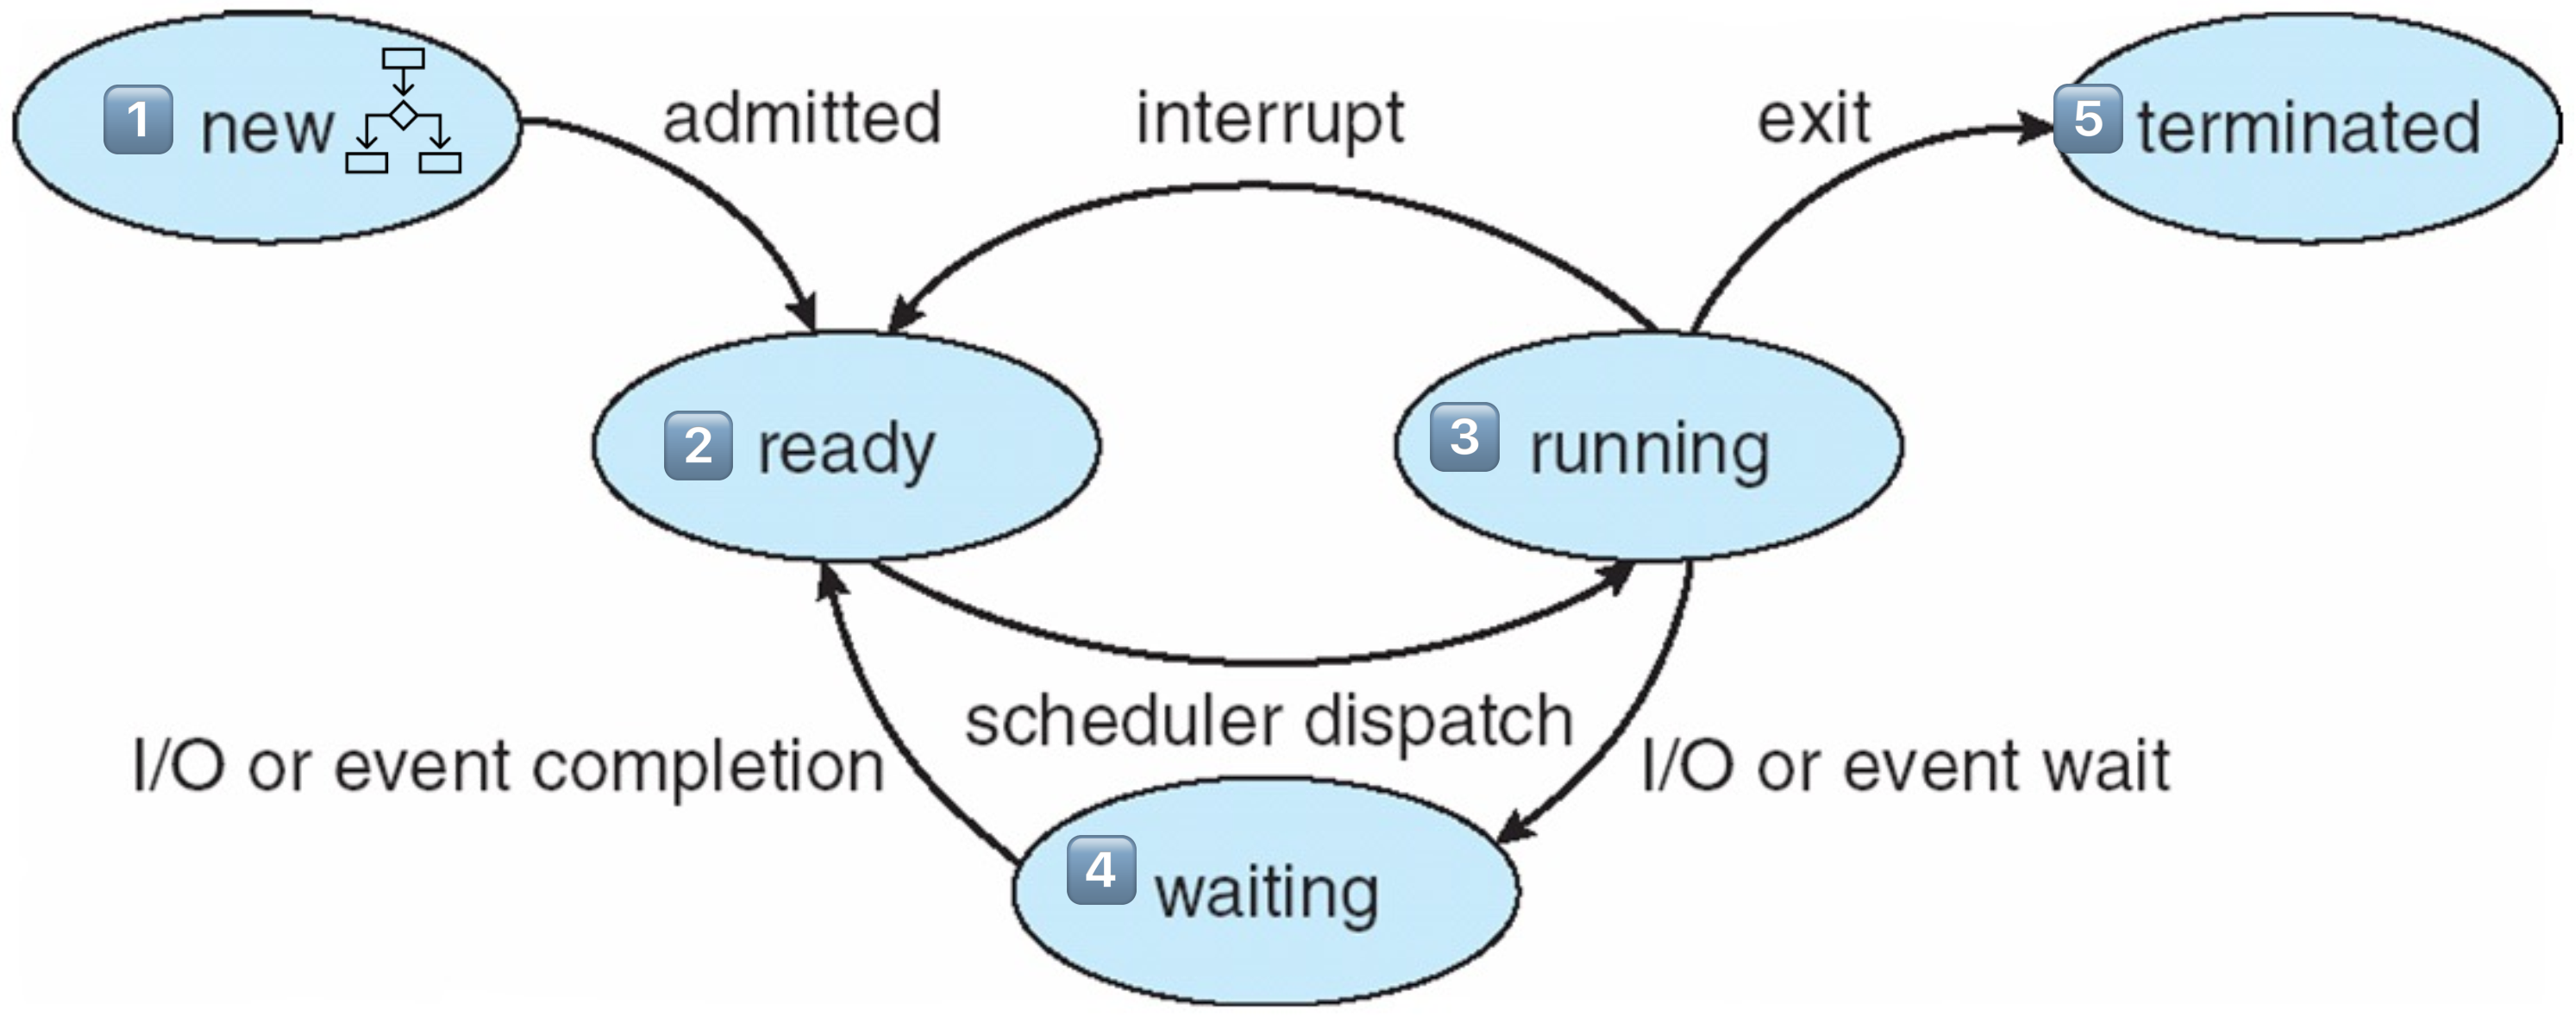
\includegraphics[width=0.95\linewidth]{images/03a_p09_process_states.png}

\textbf{Process scheduling} maximizes CPU utilization via multiprogramming/time-sharing. Processes are in the ready queue (waiting for CPU) or the wait queue (blocked on I/O or events). The \textbf{CPU scheduler} (short-term) selects processes for execution, while the \textbf{job scheduler} (long-term) controls degree of multiprogramming. The \textbf{medium-term scheduler} reduces load by suspending/resuming processes.

Processes can create other processes (forming a tree) with a unique PID. A child may inherit resources, execute concurrently or after the parent, share or copy address space. A process exits by \texttt{exit()} (parent may \texttt{wait()} for termination); a parent may \texttt{abort()} a child. Orphans are avoided by cascading termination. A \textbf{zombie} is a terminated child not yet \texttt{wait()}-ed for.

\textbf{Interprocess communication (IPC)} allows cooperating processes to share info. Two main models: \textbf{shared memory} (fast, but requires synchronization like producer-consumer patterns) and \textbf{message passing} (explicit send/receive, fixed or variable-sized messages, with links that can be direct or via mailboxes). IPC can be blocking (synchronous) or non-blocking (asynchronous); buffering can be zero, bounded, or unbounded. Examples: \textbf{pipes} (ordinary: parent-child only, named: general access) and \textbf{sockets} (for client-server comms, using TCP or UDP).


\subsubsection*{3b) Threads and Concurrency}

A \textbf{thread} is the smallest unit of CPU execution within a process. Threads share code, data, and OS resources but have independent program counters, registers, and stacks. Thread creation is lightweight compared to processes, enabling higher efficiency. Benefits include responsiveness, resource sharing, scalability, and simplified communication.

\textbf{Concurrency} (multiple tasks make progress) is interleaving execution of multiple tasks (sw). \textbf{Parallelism} is simultaneous execution of multiple tasks on multiple cores (hw). Modern CPUs have multiple cores, supporting both concurrency and parallelism. Work can be distributed by \textbf{data parallelism} (split data across threads) or \textbf{task parallelism} (split tasks).

\textbf{Amdahl's Law} estimates speedup from parallelization: $Speedup = 1 / (S + (1-S)/N)$, where $S$ is the serial portion.
Ignores parallelization overhead (e.g., task creation, contention, synchronization).
Serial portion limits speedup.

\textbf{(UT)}: managed in user space, invisible to kernel.
\textbf{(KT)}: managed and scheduled by kernel.

Thread models: \textbf{N:1} (many UT map to one KT), \textbf{1:1} (each UT has its own KT), and \textbf{M:N} (many UT multiplexed over KT). Some systems use a \textbf{Two-Level} model (hybrid of M:M with dedicated mappings).

% Thread model implications:
\textbf{N:1}: Blocking one user thread blocks all (only one kernel thread).
\textbf{1:1}: Higher concurrency, but thread count per process may be limited (kernel overhead).
\textbf{M:N}: Kernel can schedule another thread if one is blocked; avoids N:1 problem.
\textbf{Two-Level}: Some user threads have dedicated 1:1 mapping (e.g., for real-time or priority tasks).


Threads can be \textbf{explicit} (managed via API like Pthreads) or \textbf{implicit} (created by compilers/runtime). Thread \textbf{pools} pre-create threads for efficiency. \textbf{OpenMP} supports implicit parallelism via compiler directives in shared memory environments.

Thread issues: \textbf{fork/exec} behavior differs (fork duplicates, exec replaces). \textbf{Signals} notify processes of events (handled synchronously or asynchronously). \textbf{Thread cancellation} allows terminating threads, either asynchronously (immediate) or deferred (checked by the target thread).

\textbf{Thread-Local Storage (TLS)} gives threads private data accessible across function calls.
TLS is useful when you can't control thread creation (e.g., with implicit threading or thread pools).
\textbf{Provides data unique to each thread}, persistent across function calls (unlike local variables).


Process vs. Thread:
A \textbf{process} is a \textbf{container for resources} (e.g., memory, open files).
A \textbf{thread} is the \textbf{execution entity} with instructions and context.
Even in a single-threaded process, it's the \textbf{thread that is scheduled} by the OS.

\textbf{T vs P usage: }Threads for tasks needing \textbf{frequent communication and shared state}.
Processes for \textbf{higher separation \& security}.

Linux treats threads as processes (no strict distinction); \texttt{clone()} creates threads, \texttt{fork()} creates separate processes. Threads share resources if specified by \texttt{clone()} flags.

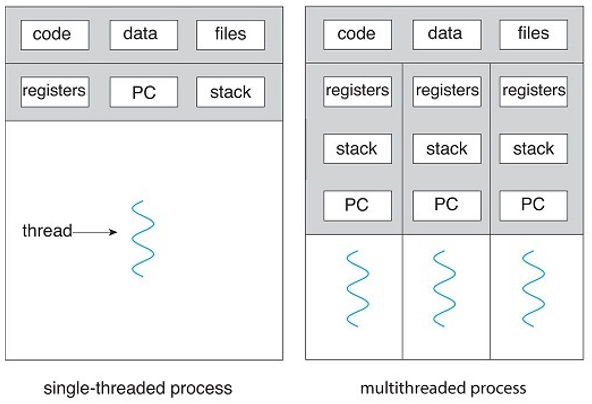
\includegraphics[width=0.95\linewidth]{images/03a_p14_threaded_process.png}

\subsubsection*{3c) CPU Scheduling}

A process alternates between CPU and I/O bursts. CPU-bound processes have few long bursts; I/O-bound processes have many short bursts. Scheduling selects which process/thread to execute: \textbf{short-term scheduler} chooses from the ready queue, \textbf{long-term scheduler} controls the degree of multiprogramming, \textbf{medium-term scheduler} may swap processes out.

\textbf{Preemptive} scheduling interrupts running processes (risk of race conditions, must handle in kernel mode). \textbf{Non-preemptive} scheduling waits for process to release CPU voluntarily. The \textbf{dispatcher} handles context switching, moving from the old to the new process, introducing latency (ideally <$10\mu$s).

\textbf{Scheduling criteria}: maximize CPU utilization, throughput (completed processes/time), minimize turnaround time (completion time - arrival), waiting time (in ready queue), response time (submission to first response).

\textbf{Algorithms}:
\textbf{FCFS} (non-preemptive): simple but poor response for short processes (convoy effect).
\textbf{SJF}: optimal (minimum average waiting), predicts next burst via exponential averaging.
\textbf{Priority}: fixed or dynamic, risk of starvation; \textbf{aging} prevents starvation by increasing priority over time.  
\textbf{RR} (round robin): time-sliced FCFS, preempts after quantum; quantum too small → overhead, too large → FCFS-like behavior.  
\textbf{MLQ} (multilevel queue): queues per priority/type, fixed scheduling per queue (e.g., RR for foreground, FCFS for background), may starve lower-priority queues.
\textbf{MLFQ}: feedback mechanism allows movement between queues; short bursts → high priority, long bursts → demoted. Most flexible but complex.
\textbf{CFS} (Completely Fair Scheduler, Linux): proportional fair share; tasks with lower \texttt{vruntime} get CPU, stored in a red-black tree (O(log n)); preemptive, priority via \texttt{nice} value. Real-time tasks (0-99) have static priority, normal tasks (100-139) get dynamic fair share.

\textbf{Thread scheduling}: threads (user or kernel-level) compete within the process (\textbf{PCS}) or system-wide (\textbf{SCS}); kernel threads scheduled by OS (one-to-one model), user threads by library (many-to-one/many-to-many).  

\textbf{Multiprocessor scheduling}: cores can share queues or have per-core queues (better affinity). Load balancing via \textbf{push} (force move) or \textbf{pull} (steal work). \textbf{Processor affinity}: keeps threads on the same core for cache locality (soft/hard affinity). \textbf{NUMA-aware scheduling} places threads near memory for lower latency. \textbf{Heterogeneous multicore systems} (e.g., big.LITTLE) mix cores of different performance/power profiles.

\textbf{Algorithm evaluation}: deterministic (static workloads), queueing models (Little's Law: $N=\lambda W$), simulations, or real system tests.
    \subsubsection*{4a) Synchronization}

Ensure data consistency \& correct execution order when multiple threads / processes access shared data concurrently. Handles ordering, timing, mutual exclusion.

\textbf{Cooperating processes} execute concurrently; \textbf{shared data} access can lead to \textbf{race conditions} (unpredictable behavior). A \textbf{data race} occurs when two+ threads access the same memory, one writes, without proper ordering. \textbf{Critical section (CS)}: only one process at a time; must ensure \textbf{mutual exclusion}, \textbf{progress}, and \textbf{bounded waiting}.  

\textbf{Peterson's solution}: for 2 processes, uses \textbf{flags} and \textbf{turn} for atomic control.

\textbf{Mutex}: acquire/release lock for CS; \textbf{spinlocks} use busy waiting, preferred for short waits on SMP (Symmetric Multiprocessing).

\textbf{Semaphores}: integer S, \textbf{wait} decrements, \textbf{signal} increments; can block processes in a waiting queue. Avoids busy waiting at app level but risks \textbf{deadlocks} and \textbf{starvation}.

\textbf{Priority inversion}: low-prio holds lock needed by high-prio. 
\textbf{Bounded}: high-prio blocked by low-prio.
\textbf{Unbounded}: mid-prio preempts low-prio, extending high-prio wait. Solved by \textbf{PIP} (priority inheritance protocol) or \textbf{PCP} (priority ceiling protocol).

\textbf{Monitors}: high-level abstraction ensuring mutual exclusion; includes \textbf{condition variables} (x.wait, x.signal) for coordination.
Only one process active in monitor at a time.
Unlike semaphores, signal() has no effect if no process is waiting. 

Problems: 1) Access without permission, 2) Never release resource, 3) Release not-held resource, 4) Request same resource multiple times.


\subsubsection*{4b) Examples}
\textbf{Bounded buffer}: producer-consumer problem, \textbf{binary/counting semaphores} or \textbf{mutex locks} solve access control.

mutex = 1;
empty = n;
full = 0;

Producer:
wait(empty);
wait(mutex);
\textit{// add item}
signal(mutex);
signal(full);

Consumer:
wait(full);
wait(mutex);
\textit{// remove item}
signal(mutex);
signal(empty);

\textbf{Philosophers}: prevent \textbf{deadlock} and \textbf{starvation}; 5 philosophers, 5 chopsticks. All grabbing left chopstick: deadlock. Avoid: allow max 4 to eat, \textbf{asymmetric solution} (odd eat directly), \textbf{condition self[i]} for permission, ensure \textbf{mutual exclusion}, but can violate \textbf{bounded waiting}.

\textbf{Linux}: pre-2.6 \textbf{nonpreemptive kernel} with small CS. Provides \textbf{atomic\_t}, \textbf{spinlocks}, \textbf{semaphores}, \textbf{mutexes}. Spinlocks avoid complex locks, deterministic; needed on \textbf{SMP} for race conditions. Spinlock: acquire = disable preemption, release = enable.

\textbf{POSIX}: \textbf{named semaphores} via \texttt{sem\_open()}, unnamed via shared memory \texttt{sem\_init()}.

\textbf{OpenMP}: \textbf{compiler directives} and API; \texttt{\#pragma omp critical} or \texttt{omp atomic} for lightweight, non-blocking synch.


\subsubsection*{4c) Deadlocks}
\textbf{Deadlock}: multiple \textbf{resources} (CPU, IO, mem), multiple instances. Process \textbf{requests} (open, allocate, wait), \textbf{uses}, then \textbf{releases} (close, free, signal). 
Example: thread1 locks A then B; thread2 locks B then A → circular wait.

\textbf{Livelock}: process proceeds but no progress, often due to lock contention.
Analogy: Two people in a hallway stepping side to side, never passing.
Solution: Add randomness/asymmetry (like dining philosophers) to break the cycle.
Deadlock = waiting indefinitely. Livelock = doing actions repeatedly but no progress.

In multithreading: mutex via \texttt{pthread\_mutex\_t}, use \texttt{\_init}, \texttt{\_lock}, \texttt{\_unlock}. DL occurs when one locks first and second locks second, circular blocking.

\textbf{DL conditions}
(Only if all four conditions are present, deadlock may occur)\\
- \textbf{Mutual exclusion}: Some resources can only be held by one process at a time.\\
- \textbf{Hold \& Wait}: A process holding at least one resource is waiting for additional resources held by other processes.\\
- \textbf{No preemption}: Resources can't be forcibly taken; they must be released voluntarily.\\
- \textbf{Circular wait}: A circular chain of processes exists, each waiting for a resource held by the next one in the chain.\\

DL handling:\\
1. Prevention/Avoidance (protocols)\\
2. Detection \& Recovery\\
3. Ignore (programmer responsible) 

Prevention: break 1 of 4 conditions. \textbf{1. Mutual exclusion} (can't), \textbf{2. Hold \& wait} (request all at once), \textbf{3. Preemption} (release all on failure, often impractical), \textbf{4. Resource ordering} (unique int IDs, acquire in order).

    \subsubsection*{5a) Main Memory}
Processes loaded from disk into memory, logical (virtual) vs. physical address: CPU generates logical addresses, MMU translates to physical (relocation register adds offset). Contiguous allocation: each process occupies a single, continuous memory block. Problems: external fragmentation (holes), internal fragmentation (wasted space). Fit algorithms: first-fit, best-fit, worst-fit. Solutions: compaction, paging.  
\textbf{Paging:} Divide logical/physical memory into fixed-size pages/frames (power of 2). Page table maps page \texttt{p} to frame \texttt{f}. Logical address: (p,d), physical: (f,d). TLB caches page table entries. Protection: read/write/execute, valid/invalid bits. Shared pages for libraries. Page table structures: flat (small systems), hierarchical (multi-level page tables), hashed, inverted.  
\textbf{Swapping:} Move process or pages between RAM and disk (swap space). Supports oversubscription, thrashing risk. Roll-in/out (whole processes), or page-based swapping (demand paging). Swap triggers when memory pressure increases.

\subsubsection*{5b) Virtual Memory}
Allows larger logical address space than physical. Programs partially loaded (demand paging). OS + MMU load pages on-demand, invalid/valid bits track page status. On page fault: trap, find frame, swap page in, update page table, restart. Copy-on-write (COW) on fork: pages shared until written.  
\textbf{Page replacement:} Find victim frame when no free frame. Algorithms: FIFO (Belady anomaly), OPT (ideal, not implementable), LRU (approximates OPT).  
\textbf{Frame allocation:} Equal, proportional (process size/priority), global (all frames), or local (per-process). Global replacement risks trashing (processes competing for frames). Thresholds: low → kernel reclaims; high → suspend reclamation.  
\textbf{Trashing:} Excessive page faults due to overcommitment. Locality model: processes use working sets of pages. Working set model: \(\Delta\)-window tracks recent page usage; sum of working set sizes \(D\) must fit in RAM. If \(D\) exceeds available frames → suspend processes.  
\textbf{Linux:} Global replacement, page lists (active/inactive), kswapd (background page-out daemon). NUMA systems: allocate memory near CPU for efficiency.
    \subsubsection*{6a) File System Interface}
FS = abstraction: stores data+progs, hides phys. storage. File = ADT by OS: seq of records (bytes/lines/etc.), e.g., ELF. User view: smallest unit on disk. Attributes: name, id, type, loc (ptr), size, timestamps, perms. Pos ptr per process for R/W; all ops (exc. create/del) $\to$ open.\\
Ops: create (alloc+dir), open (name+perms), read/write (handle), seek, delete (free), truncate.\\
Access: seq (read\_next, write\_next), direct (read(n), write(n)), indexed (index in RAM).\\
Dir: single-level (global list), 2-level (per user), tree (abs/rel path), acyclic-graph (links$\to$files, resolve). Dir+files = on disk. No cycles: file-only links, GC, or detect on link add. Dir ops: search, create, delete, list, rename, traverse.\\
Mem-mapped = alt to syscalls (open/R/W); shared mem via mmap.

\subsubsection*{6b) FS Implementation}
FS enable access to storage (disks/NVM). Disks: blocks w/ sectors (512/4096 B).
FS design balances UI \& algorithms mapping logical FS to physical. Layered arch.: app → logical FS (metadata, dirs, FCBs) → file org (files, logical blocks, free space) → basic FS → I/O ctrl → device drivers/interrupts. Pseudo-FS (e.g., /proc in Linux, at /proc) = virtual FS in kernel mem, file interface for system info (e.g., /proc/cpuinfo, /proc/[pid]/status, /proc/meminfo), contents generated on access. Pseudo-FS $\neq$ Gen-FS: no backing store, dynamic data, mostly r/o. Gen-FS: persistent, modifiable.  
FS types: UNIX FS, NTFS, FAT, ext3/4.  
On-disk/in-mem data: boot block (bootloader = blocks loading kernel from FS), volume ctrl block (superblock/MFT: \#blocks, block size, free-block count/pointers), dirs, FCBs. Mount = attach volume (e.g., /dev/sda1) at mount point (dir); volumes may span partitions (e.g., LVM). Mounting checks valid FS via device driver reading device dir.  
Caches: dir info, open file tables (global + per-process w/ FCBs), block buffers.  
Name lookup: linear list (slow), hash table (faster, collisions), ordered list (linked), B+ trees.  
Block alloc: contiguous (fast, needs size, external frag, compaction), linked (pointers, no external frag, sequential access), indexed (index block(s), random access, overhead, handles via linked/multilevel/combined).  
Free-space mgmt: bitmap (bit=free/used), free list (linked blocks, no contiguous alloc), grouping (list of free blocks per block).

\subsubsection*{6c) FS Internals}
Storage devices split into partitions (e.g., /dev/sda1), each mountable as a volume (FS-formatted). Raw partition = no FS; cooked = has FS. Root partition: OS, bootloader specifies (loads kernel from FS). Other partitions: other OS, FS, user data; mounted auto/manual (e.g., /dev/sda1 at /home).  
Mount = associate volume w/ mount point (dir in tree). Volumes must be mounted before access; OS verifies FS via device driver.
    \subsubsection*{7) Virtualization}
\textbf{Virtualization:} abstraction of \textbf{hardware} (CPU, mem, I/O) for multiple isolated \textbf{environments (VMs)}. Overcomes \textbf{multicomputer model} limits (standalone machines) by combining reliability, isolation (sandboxing), and flexibility.

\textbf{Components:} \textbf{Host} (HW), \textbf{Hypervisor (VMM)} (creates/manages VMs), \textbf{Guest} (process with virtual HW view).

\textbf{Types:} \textbf{Type 0} (\textbf{firmware partitions/domains}), small feature set. \textbf{Type 1} (native, datacenters, e.g., \texttt{ESXi}), runs in kernel mode, manages OSes, snapshots, cloning, balancing load. \textbf{Type 2} (hosted, e.g., \texttt{VirtualBox}), runs as a process on host OS, higher latency. Compare: \textbf{Type 1} → low latency, needs HW support, service providers; \textbf{Type 2} → high latency, no HW req., end-users.

\textbf{Building Blocks:} \textbf{VCPU} stores guest state, switched by VMM. \textbf{HW support} essential (e.g., \texttt{Intel VT-x}, \texttt{AMD-V}), incl. nested page tables, DMA, interrupts. \textbf{Trap \& Emulate:} guest runs in \textbf{virtual user/kernel mode} (both in HW user mode); traps on priv. instr. \textbf{Binary Translation:} rewrites priv. instr. on CPUs w/o clean separation. \textbf{Emulation:} simulates different ISA, slow.

\textbf{Paravirtualization:} modify guest OS to avoid traps.

\textbf{Programming Env VM:} e.g., \texttt{JVM} abstracts exec. env., cross-OS portability.

\textbf{Containers:} App-level isolation via \textbf{OS namespaces}; each has own FS, net stack, users. Lightweight, fast start, no full OS. \textbf{Docker}: \textbf{Image} (layers: e.g., Ubuntu, Python), \textbf{Container} (instance), \textbf{Engine}, \textbf{Registry}. Shared layers reduce redundancy. Compare VMs vs Containers: \textbf{VMs} heavy, slow, full OS, hardware virt.; \textbf{Containers} light, fast, process-level isolation, share OS.

\textbf{CPU Scheduling:} VMM schedules VCPUs on physical CPUs; \textbf{overcommit} = more VCPUs than CPUs.

\textbf{Memory Mgmt:} VMM mediates guest/host mem; uses nested page tables. \textbf{Overcommit:} total guest alloc > physical mem. VMM uses own paging, replacement.

\textbf{Storage:} VMs see \textbf{disk images} (Type 1 = VMM FS, Type 2 = host FS). \textbf{P2V/V2P} convert disk formats. VMM handles net disks.

\textbf{Live Migration:} Copy running VM incl. CPU state, memory pages (iterative dirty page copy); no disk state. \textbf{MAC mobility} requires network switch support.

\textbf{Container Problems Solved:} \textbf{VM CapEx/OpEx} (licenses, OS overhead) → Containers = low-cost, fast deploy. \textbf{Application Containment:} consistent, portable env; auto-packages apps + dependencies.

    \subsubsection*{8) OpenMP \& Parallelization}
Parallelization maps computation on data to parallel/distributed systems respecting dependencies. Key steps: analyze program parallelism, identify \textbf{task/data parallelism}, decompose \textbf{granularity} (fine, medium, coarse), and consider communication cost.

Dependencies: \textbf{control} (task order), \textbf{data} (flow, anti, output), \textbf{name} dependencies. Mapping: assign subtasks spatially (processor) and temporally (when), \textbf{static/dynamic} scheduling.

OpenMP: \textbf{shared-memory API} for multi-threading via \#pragma omp, runtime libs, env vars (OMP\_NUM\_THREADS). \textbf{Simplifies} parallel code, portable across multicore, NUMA, GPUs. Parallel regions execute copies of code; loops via \#pragma omp parallel for. Threads share vars, needing \textbf{synchronization} (critical, atomic, barriers) to avoid \textbf{races}. Functions: \texttt{omp\_set\_num\_threads()}, \texttt{omp\_get\_thread\_num()}, \texttt{omp\_in\_parallel()}, \texttt{omp\_get\_num\_procs()}, \texttt{omp\_set\_dynamic()}. Use \textbf{private}, \textbf{shared}, \textbf{reduction} clauses.

Limitations: OpenMP is \textbf{shared-memory only}, lower parallel efficiency vs MPI for distributed memory.
Performance: needs enough parallelism, balanced load, data locality, minimize synchronization.
Overhead: communication, cache effects, false sharing, load imbalance.
Tools: \textbf{OMP\_NUM\_THREADS}, \textbf{OMP\_SCHEDULE}, \textbf{parallel loops}, critical sections, \textbf{barriers}.

\textbf{Speedup limit:} Amdahl’s Law $S = 1 / (f + (1 - f) / N)$ (f=serial fraction). \textbf{Scalability:} impacted by sequential part, load imbalance, communication.

    % \columnbreak
\end{multicols}

\end{document}